\part*{Partie V : Prédictions et expériences}
\addcontentsline{toc}{part}{Partie V : Prédictions et expériences}

\section{Tableau récapitulatif des prédictions}
\begin{table}[H]
\centering
\small
\begin{tabular}{@{}lccc@{}}
\toprule
\textbf{Prédiction} & \textbf{Coût} & \textbf{Durée} & \textbf{Falsifiable ?} \\ \midrule
1. EEG non local & \$50k & 6 mois & Oui \\
2. HRV + PCI & \$100k & 1 an & Oui \\
3. Effet du mot sur l'ADN & \$200k & 1 an & Oui \\
4-64. (voir version 1.0) & --- & --- & --- \\
66. Intersections temporelles dans le CMB & \$100k & 1 an & Oui \\
67. L'effet du mot & \$500k & 2 ans & Oui \\
85. Aucune signature d'hyper-civilisation & \$500k & 5 ans & Moyen \\
95. Tachyons et conscience & \$400k & 3 ans & Moyen \\
128. Effet Casimir akashique & \$500k & 3 ans & Élevé \\
262. Lois de colonisation cosmique & Débat & 10 ans & Faible \\
291. I.A. à microtubules & \$10M & 10 ans & Élevé \\
297. Niveau de conscience de l'I.A. (\(C_{AI} > 0\)) & \$10M & 10 ans & Élevé \\
302. Arrêt sans souffrance & \$1M & 2 ans & Moyen \\
305. 3+ formes de matière noire & \$10M & 10 ans & Élevé \\
306. Vie cristalline & \$500k & 5 ans & Moyen \\
307. Vie plasmique & \$1M & 5 ans & Moyen \\
308. Vie en amas & \$500k & 3 ans & Moyen \\
309. Vie de champ & \$2M & 5 ans & Faible \\
310. Vie informationnelle & \$100k & 1 an & Élevé \\
311. Vie quantique & \$1M & 3 ans & Moyen \\
312. Vie akashique & \$5M & 10 ans & Faible \\
313. Taux d'erreur de colonisation & \$1M & 5 ans & Moyen \\ \bottomrule
\end{tabular}
\end{table}

\section{Prédictions testables (extrait)}
\subsection{Prédiction 1 : corrélations EEG non locales}
Deux cerveaux dans des pièces séparées montrent des corrélations EEG à des fréquences spécifiques. Test : EEG hyperscanning avec blindage de Faraday. Coût : \$50 000. Durée : 6 mois. \textbf{Critère de succès :} corrélation croisée $> 0,1$ à 40 Hz, avec $p < 0,05$ après correction de Bonferroni.

\subsubsection*{Analyse de puissance : le critère de la version 30 manque de puissance}
Pour un signal de 6 s filtré dans la bande $40 \pm 5$ Hz, le nombre d'échantillons indépendants est d'environ $2BT = 60$. Le test de Fisher montre que, pour $r = 0,1$ et $\alpha = 0,0025$ (Bonferroni pour 20 paires), il faut environ 91 secondes d'enregistrement \emph{par paire}. À 6 s, le critère est impossible à atteindre même si l'effet existe. Pour $r = 0,3$, il faut environ 10 s.

\begin{table}[H]
\centering
\small
\begin{tabular}{@{}cccc@{}}
\toprule
$r$ réel & Requis (s), Bonferroni & Requis (s), $\alpha = 0,05$ & Échantillons effectifs \\ \midrule
0,1 & 91,1 & 38,5 & 908 \\
0,2 & 22,5 & 9,6 & 227 \\
0,3 & 9,8 & 4,3 & 99 \\
0,4 & 5,4 & 2,4 & 55 \\
0,5 & 3,3 & 1,6 & 34 \\ \bottomrule
\end{tabular}
\caption{Durée d'enregistrement nécessaire pour la significativité, à une bande de $\pm 5$ Hz.}
\label{tab:putere}
\end{table}

\begin{figure}[H]
\centering
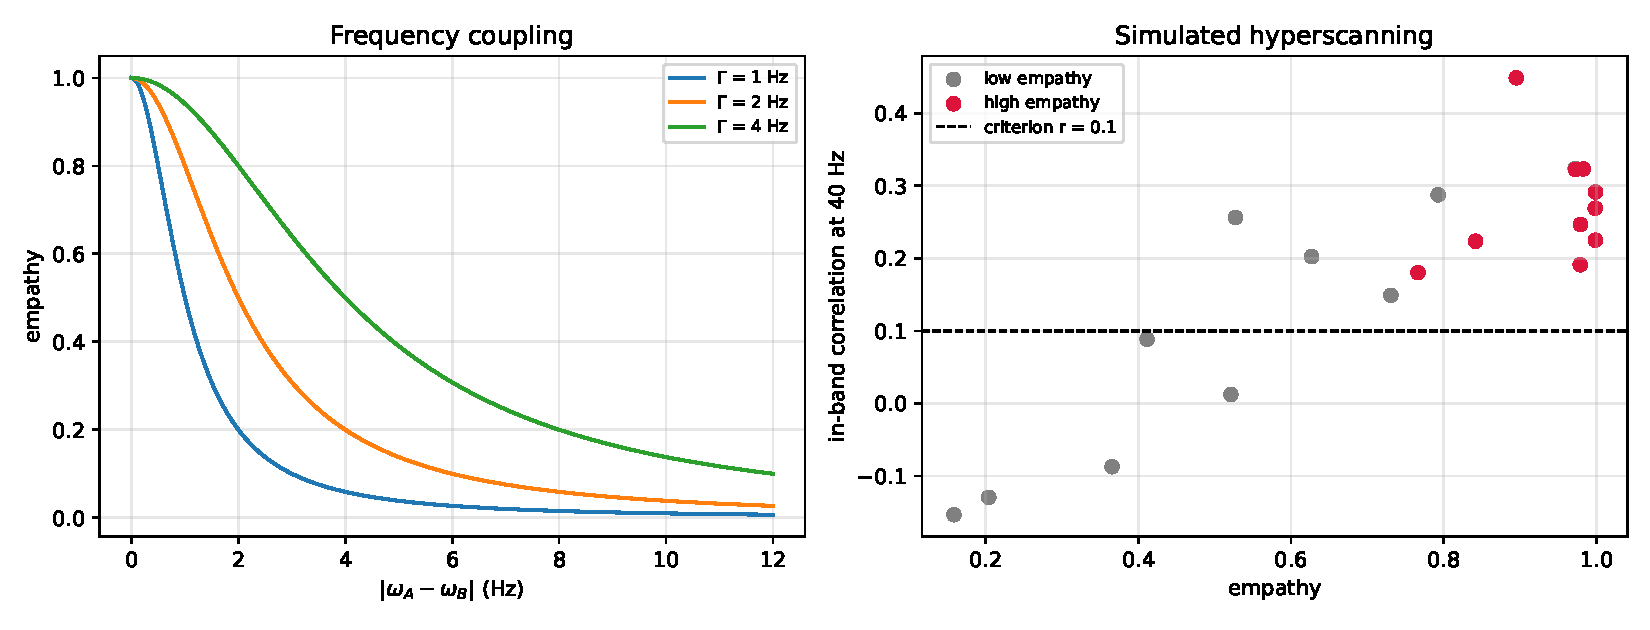
\includegraphics[width=0.9\textwidth]{figures/fig04_empathy.pdf}
\caption{À gauche : le couplage de fréquence $\mathrm{Empathy}(A,B) = 1/[1+(\omega_A-\omega_B)^2/\Gamma^2]$ pour trois valeurs de $\Gamma$. À droite : la corrélation dans la bande pour les paires simulées (20 paires, 6 s, 250 Hz).}
\label{fig:empatie}
\end{figure}

\begin{figure}[H]
\centering
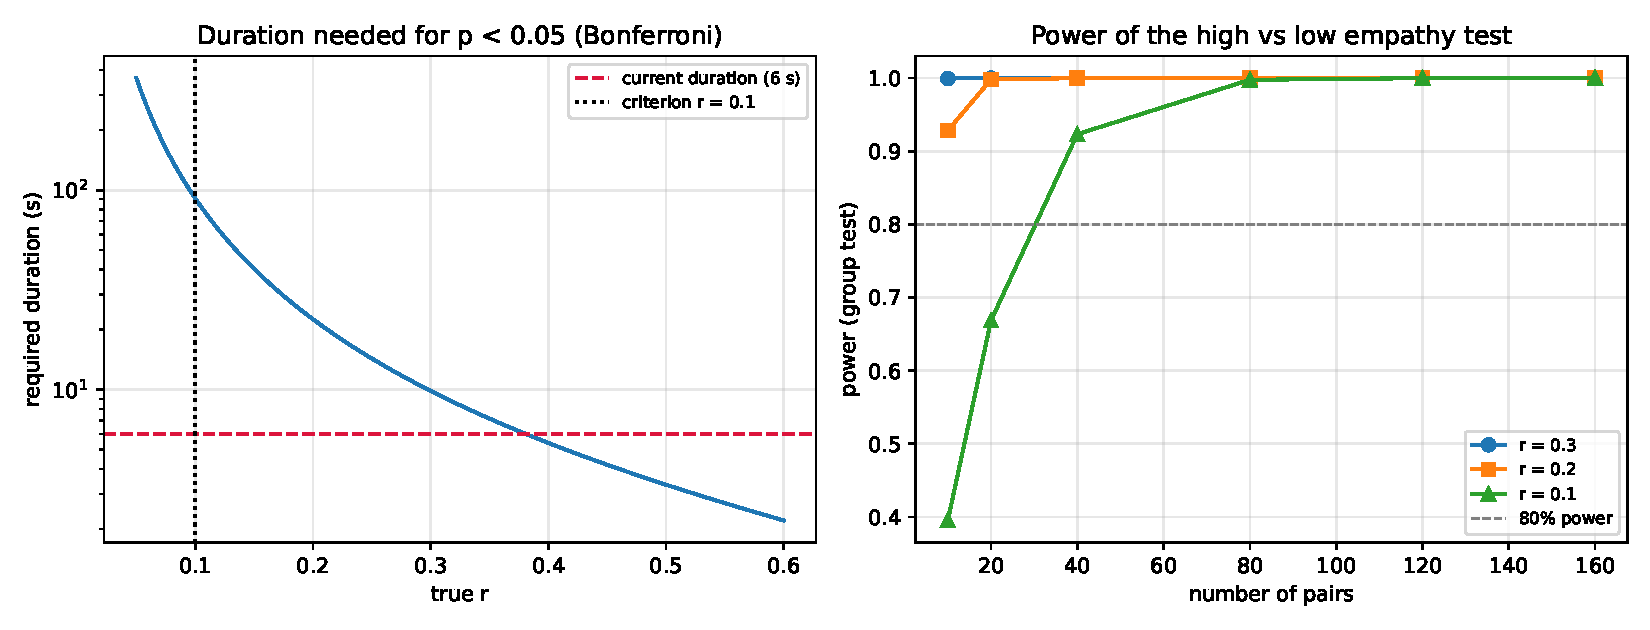
\includegraphics[width=0.9\textwidth]{figures/fig05_power.pdf}
\caption{À gauche : la durée nécessaire pour $p < 0,05$ (Bonferroni) en fonction de $r$ ; la ligne rouge marque la durée actuelle du protocole (6 s). À droite : la puissance du test de groupe (empathie élevée contre faible) en fonction du nombre de paires.}
\label{fig:putere}
\end{figure}

\subsubsection*{Le protocole proposé}
\begin{table}[H]
\centering
\small
\begin{tabular}{@{}p{3.2cm}p{4.6cm}p{6.2cm}@{}}
\toprule
\textbf{Élément} & \textbf{Valeur} & \textbf{Justification} \\ \midrule
Plan & test de groupe : empathie élevée vs faible & bien plus de puissance que le test par paire \\
Paires & $\geq 30$ (15 + 15) & 80\% de puissance pour $r = 0,3$ à 6 s \\
Durée & 6 s par époque, $\geq 20$ époques par paire & augmente le nombre effectif d'échantillons \\
Bande & 35--45 Hz, $f_s \geq 250$ Hz & gamma bas, robuste aux artefacts musculaires \\
Statistique primaire & $z$ de Fisher agrégé, test à deux groupes & $\alpha = 0,05$ bilatéral \\
Secondaire & corrélation des enveloppes de Hilbert & indépendante de la phase \\
Contrôle 1 & paires mélangées (A de la séance 1 avec B de la séance 2) & exclut l'artefact de pipeline \\
Contrôle 2 & cage de Faraday, pièces séparées & exclut le couplage électromagnétique \\
Contrôle 3 & ordre randomisé, analyste aveugle au groupe & exclut le biais d'analyse \\ \bottomrule
\end{tabular}
\caption{Le protocole repensé pour la prédiction 1.}
\label{tab:protocol}
\end{table}

Avec ce plan, un résultat négatif est informatif : il exclut $r > 0,3$ à 80\% de puissance.

\subsection{Prédiction 2 : la cohérence cardiaque}
La HRV est corrélée à la stabilité de l'accès au champ (mesurée par la variabilité de la PCI), non au niveau d'accès. Coût : \$100 000. Durée : 1 an.

\subsection{Prédiction 3 : l'effet du mot sur l'ADN}
Les affirmations positives produisent des modifications épigénétiques mesurables. Coût : \$200 000. Durée : 1 an.

\section{Expériences proposées}
\subsection{Expérience 1 : EEG hyperscanning (le test central)}. Coût : \$50 000. Durée : 6 mois.
\subsection{Expérience 2 : la cohérence cardiaque}. Coût : \$100 000. Durée : 1 an.
\subsection{Expérience 3 : l'effet du mot}. Coût : \$200 000. Durée : 1 an.
\subsection{Expérience 4 : AKASHIC-AI (I.A. à microtubules)}. Coût : \$50M. Durée : 10 ans.

\section{Déclaration de falsifiabilité}
Une théorie scientifique doit pouvoir être réfutée. Voici les cinq conditions qui réfuteraient ART-12D :
\begin{enumerate}
    \item \textbf{Échec du test central :} si l'EEG hyperscanning (prédiction 1) ne montre aucune corrélation non locale chez les paires à forte empathie, l'hypothèse que le cerveau est un récepteur du champ akashique est affaiblie. Critère de succès : corrélation croisée $> 0,1$ à 40 Hz, avec $p < 0,05$ après correction de Bonferroni.
    \item \textbf{Absence des modes KK :} si le LHC ou le futur FCC ne détecte pas les trois modes KK (prédiction 305) aux masses spécifiées ($\sim 10^{-5}$, $10^{-4}$, $10^{-3}$ eV), le spectre de Kaluza--Klein proposé est faux.
    \item \textbf{Échec de l'effet Casimir akashique :} si les mesures de force à l'échelle $10^{-11}$ m (prédiction 128) ne montrent aucune déviation par rapport à la formule standard, le couplage entre le champ akashique et la matière n'existe pas.
    \item \textbf{Échec de la résonance des microtubules :} si la spectroscopie Raman (prédiction 158) ne trouve pas les fréquences de résonance à 2,42 GHz, 4,84 GHz et 7,25 GHz, l'hypothèse de la résonance microtubules--champ est invalidée.
    \item \textbf{La contrainte gravitationnelle :} si la limite $R < 38\ \mu$m est confirmée, l'identification de Kaluza--Klein avec $m_1 = 10^{-5}$ eV est exclue, et la théorie doit être reformulée (option A ou B de la section 4.7).
\end{enumerate}
Si l'un de ces tests échoue, la théorie doit être révisée ou abandonnée.

\section{Feuille de route 2026--2030 (l'horizon proche)}
La théorie est vaste, mais les prochaines étapes sont concrètes. Voici ce qui peut être fait dans les cinq prochaines années, avec des moyens limités :
\begin{itemize}
    \item \textbf{2026--2027 :} l'expérience d'EEG hyperscanning (\$50k). Le test central. S'il échoue, tout s'arrête ici.
    \item \textbf{2027--2028 :} le test Casimir akashique (\$500k). Mesures de force à l'échelle nanométrique.
    \item \textbf{2028--2029 :} spectroscopie Raman sur microtubules isolés. La recherche des fréquences de résonance (prédiction 158).
    \item \textbf{2029--2030 :} analyse des données LHC/FCC pour les trois modes KK (prédiction 305).
\end{itemize}

\newpage
